\section{Join Ordering}
Join ordering focuses on conjunctive queries with simple predicates of the type $a_1 = a_2$ where the latter can be either an attribute or a constant (commonly algorithms assume join between attributes).

Relations may include selections or complex building blocks, however for simplicity filtering is ignored; having operators other than equality might cause differences within the query planner.

Ordering basically means choosing which relation to be joined first, placing entities in a graph and adding an edge whenever a predicate from a node is joined to another. 

This kind of schema is defined as a query graph, in which edges consist in predicates and self loops represent equality with a constant. Usually cycles are pushed down, since algorithms only assume attributes. 

Based on the query graph it is possible to obtain an overview of the complexity of the problem: there are different shapes which are treated differently. 

\begin{figure}[h]
	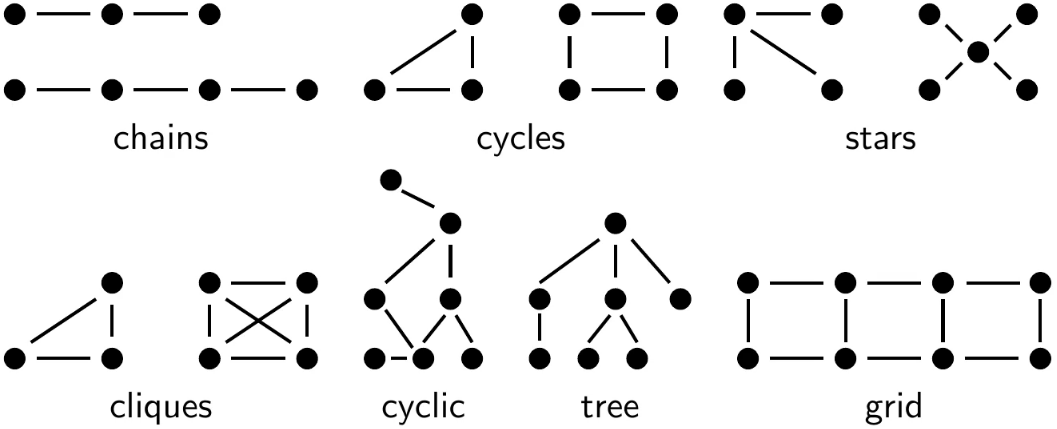
\includegraphics[scale=1.5]{query_graph.png}
	\centering
\end{figure}

\begin{enumerate}
	\item Chains are the simplest kind of query, fairly common in practice;
	\item Cycles (cyclic) are a chain with a closing edge, the easiest example of cycles;
	\item Stars are mostly used in data warehouse, in which the center table has large dimension and the ones outside are relatively small, quite different to solve;
	\item Cliques are instances in which every relation is joined with all the others, and are the hardest to optimize causing the worst runtime;
	\item Trees are acyclic queries even if the level of nesting can be high;
	\item Grids are also fairly hard and interesting for research.
\end{enumerate}

Joins are represented with join trees, binary trees with operators as inner nodes and relations as leaves. The most common type is unordered (not distinguish left from right) without cross product, however algorithms might produce other variants.

There furthermore are different kinds of trees:
\begin{itemize}
	\item Left-deep tree, in which joins only happen on the left side, easy to represent and implement through hash tables ($n!$ trees with cross products);
	\item Right-deep tree ($n!$);
	\item Zig-zag tree, a combination of the previous ($n!2^{n-2}$);
	\item Bushy tree, a full binary tree (non-linear, harder to find optimal solutions but can be the most efficient in some cases, $n!C(n-1) = \frac{(2n-2)!}{(n-1)!}$ where $C$ represents a Catalan number).
\end{itemize}
It is relevant to notice that the number of leaf combinations and unlabeled trees grows exponentially, and increases even more with a flexible structure. However, nodes can often be swapped from left to right.

Another important information about joins is their selectivity: 
$$f_{i, j} = \frac{\abs{R_i \bowtie_{p_{i, j}} R_j}}{\abs{R_i \times R_j}}$$
This depends on whether the attributes are a key, and gives an estimation of the result cardinality with the aid of assumptions and statistics.

Given a join tree, the cardinality can be computed recursively as the productory of the selectivity function multiplied by the size of both relations. This allows easy calculations only requiring base cardinalities and independence of predicates:
$$C_{out}(T) = \begin{cases}
0 & T\text{ is a leaf} \\
\abs{T} + C_{out}(T_1) + C_{out}(T_2) & T = T_1 \bowtie T_2
\end{cases}$$
This formula sums up the sizes of intermediate results, which are the ones causing more works. There are basic specific cost functions for joins, to be summed to the cost of single relations. 

Algorithms are mainly designed for left-deep trees, and some of the cost functions do not work in practice, for instance in the case of cross products. Therefore, those indicators are mainly theoretical and work under strict assumptions. However, join ordering is a main factor regardless of the chosen cost methods.

A cost function is called symmetric if $C_{impl}(e_1 \bowtie^{impl} e_2) = C_{impl}(e_2 \bowtie^{impl} e_1)$. Commutativity can be ignored.

Most of the time, algorithms for query optimization tend to avoid cross products, despite the enormous number of possibilities to build a join tree: the only exception regards small relations.

\subsubsection{Chains}
Chains usually originate a left-deep tree: leaves can be ordered according to different degrees of freedom, as long as all the relations are joined. 

The number of possible left-deep trees can be defined recursively:
$$\begin{cases}
f(0) = 0 \\
f(1) = 1 \\
f(n) = 1 + \sum_{k=1}^{n-1} f(k-1) \cdot (n - k)
\end{cases}$$
Adding $R_n$ to all possible join trees can be done at any position following $R_{n-1}$. There are $n - k$ join trees for $R_n$, plus one assuming it can be placed before $R_{n-1}$ in the case of $k=1$. For $R_{n-1}$ to be at $k$, $R_{n-k} - \dots R_{n-2}$ must be below it.

Solving the recurrence gives the closed form $f(n) = 2^{n-1}$, still exponential yet much less than the case with cross products.

A generalization to zig-zag can be made expecting the same result.

Bushy trees, on the other hand, are not so easy to obtain: each subtree must contain a subchain to avoid cross products, hence single relations should not be added. It is possible to create a whole chain $R_1 - \dots R_n$, cut it and place it under another subtree, always considering commutativity.

This gives the formula:
$$ f(n) = \begin{cases}
1 & n < 2 \\
\sum_{k=1}^{n-1} 2f(k) \cdot f(n-k) & n \geq 2
\end{cases}$$
Having more than 2 relations implying performing a cut at some point $k$ and placing $k$ on the left side, $n - k$ on the right side. A factor of 2 indicates swapping the two sides. 

This gives the closed form $f(n) = 2^{n-1}C(n-1)$.

\subsubsection{Stars}
Star queries have the constraint that one relation must be in the center; all the others can be ordered arbitrarily. This leads to the following formulas:
\begin{itemize}
	\item Left-deep: $2 \cdot (n - 1)!$, since there are $n - 1$ choices for a join partner and a factor of 2 for commutativity;
	\item Zig-zag: $2 \cdot (n - 1)! \cdot 2^{n-2}$, in which the last factor represent the possibility to swap left and right for each subtree;
	\item Bushy trees: not possible since they require the first relation to be available. 
\end{itemize}

\subsubsection{Cliques}
Cliques are a schema which do not care about cross products, since every relation is connected to the other, hence the number of possibilities is the same as the one obtained allowing cross products. 

Still, complexity is very high and runtime is bad, although the worst case usually does not happen. 

\subsection{Greedy heuristics}
Regardless of the methods and the inclusion of cross products, the search space is in general quite large when the number of relations is larger than 10, and polynomial time is hard to achieve. Some cost functions do not even have a proof of complexity.

Due to the size of the search space, greedy heuristics are ways to easily construct a potential tree in a fast time: they are most suitable for large queries, but often do not give the best result.

Algorithms assume no cross products within left-deep trees, and known cardinalities (or some other weight function).

\subsubsection{GreedyJoinOrdering-1}
This algorithm returns a set of ordered relations to be joined according to a cost function in a bushy tree structure. 

The output is given starting from the minimum-weight relation, removes it and searches for the new minimum. 

This method is simple, but not that good in practice: it assumed fixed weight (not depending on the size, for instance) and does not support optimization within intermediate results. 

\subsubsection{GreedyJoinOrdering-2}
This variant also considers the previous set of relations, computing relative weights based on the existing tree. 

In this case, however, the very first relation has a large relative weight and a major impact on the choices made afterwards. 

\subsubsection{GreedyJoinOrdering-3}
To tackle this problem, a double loop is introduced in which not only the set of relations is scanned, but also every relation is tested as a starting one. Then, all computed results are compared and the minimum among them is returned. 

This method is overall the best one and is implemented in some systems, but it is still not optimal.

\subsubsection{Greedy Operator Ordering}
Intermediate join trees must be combined to obtain larger trees: since some algorithms construct left-deep structures and others return bushy trees, those can be attached if the result is minimal: trees with the smallest weight are iteratively joined and then removed by the set of possibilities. 

First, each combination of weight (for instance, product of cardinalities and selectivity) is calculated; then the minimum is chosen and the two relations are aggregated. 

In case both relations are linked to the same (different) one in the query graph, the selectivity of the new edge consists in the product of previous ones. 

This algorithm has two pitfalls: one is its computational complexity of $O(n^3)$, which however can be in the order of milliseconds with small input, and the other is its sub-optimal output in some cases.

In fact, it is not guaranteed that Greedy Operator Ordering finds the best bushy tree given a set of relation, even if it tends to have better results than the greedy ordering techniques.

\subsection{IKKBZ}
IKKBZ is a polynomial time algorithm for join ordering without cross products, producing left-deep trees under some assumptions: acyclic graphs, ASI cost functions and a fixed join technique.

The algorithm will ultimately compute a rank for each predicate, based on its selectivity, obtaining an optimal evaluation order. After the first steps, however, the remaining arguments are independent on the size of the relations.

It starts considering a cost function as a product of the form:
$$C(T_i \bowtie R_j) = \abs{T_i} \cdot h_j(\abs{R_j})$$
Each relation $R$ can have its own $h$, which has a set of parametrized cost functions. Cardinalities are also taken into account, defining $n_i = \abs{R_i}$ and $h_i(n_i)$ as the cost per input tuple of a join. $T_i$ is the left side of the computation.

A predecende graph helps identifying which relations should be joined first; it is represented as an oriented query graph, and constructed with root in $R_k$ in the following way:
\begin{enumerate}
	\item The root is fixed, removed by the set of possibilities and added to the tree;
	\item As long as there are relations to be chosen, $R_i \in V \setminus V_k^P$ is selected such that $\exists\ R_j \in V_k^P : (R_j, R_i) \in E$;
	\item $R_i$ is added to $V_k^P$ and an edge $R_j \rightarrow R_i$ is created.
\end{enumerate}

The algorithm constructs left-deep trees.

A sequence of nodes conforms to a precedence graph if two conditions are satisfied:
\begin{itemize}
	\item For each position $i$, there exists one $j$ coming before;
	\item There does not exist a position $i$ and a $j$ coming after with an edge from $j$ to $i$ (acyclic).
\end{itemize}

If there exists a path between two sets of relations $R_i$ and $R'_i$, all relations from the first must be joined first; there is no join condition between any pair of relations aside from the one joining the two sets, hence the selectivity is 1.

Selectivity of the join:
$$s_i = \begin{cases}
1 & \abs{R_i'} = 0 \\
\prod_{R_j \in R'_i} f_{i, j} & \abs{R'_i} > 0
\end{cases}$$
In case of cycles, the selectivity cannot be uniquely determined: there could be two relations with different values. Therefore, first the precedence graph is fixed, and then selectivities are calculated.

If the query graph is a chain (total order), then the following properties hold:
$$n_{1, 2, \dots, k} = \prod_{i=1}^{k}s_in_i$$
$$C_H(G) = \sum_{i=2}^{n}\big[n_{1, 2, \dots, i-1}h_i(n_i)\big] = \sum_{i=2}^{n}\Big[\Big(\prod_{j=1}^{i}s_jn_j\Big)h_i(n_i)\Big]$$
The cardinality of the joins is equal to the productory of each selectivity for each cardinality among all relations.

If the weight function is indeed the selectivity, then $C_H \equiv C_{out}$. The factor $s_in_i$ determines how much the input relation changes its cardinality before further joins, and can be increasing or decreasing.

The algorithm employs a recursive definition of the cost function:
$$\begin{cases}
C_H(\epsilon) = 0 \\
C_H(R_i) = 0 & \text{the relation is the root} \\
C_H(R_i) = h_i(n_i) & \text{else} \\
C_H(S_1S_2) = C_H(S_1) + T(S_1) \cdot C_H(S_2)
\end{cases}$$
$$T(\epsilon) = 1 \qquad \land \qquad T(S) = \prod_{R_i \in S}s_in_i$$
Last $C_H$ definition corresponds to the cardinality performing all the relation in the sequence (the term $T$) and multiplying for the cost of last element.

This allows to use ASI properties: in fact, these hold if and only if there exists a function $T$ and a rank function defined as:
$$rank(S) = \frac{T(S) - 1}{C(S)}$$
The following must hold:
$$C(AUVB) \leq C(AVUB) \leftrightarrow rank(U) \leq rank(V)$$
In other words, ASI properties hold if and only if the relations can be ordered by rank. The cost function previously defined can be proven to respect these constraints.

It is possible that the rank contradicts the precedence graph: the following definition is introduced to counter this occurrence.

Let $M = \{A_1, \dots, A_n\}$ be a set of sequences of nodes. Then $M$ is called a module if, for all sequences $B$ that do not overlap with the sequences in $M$, one of the following conditions holds:
\begin{itemize}
	\item $B \rightarrow A_i, \forall\ A_i \in M$;
	\item $A_i \rightarrow B, \forall\ A_i \in M$;
	\item $B \nrightarrow A_i \land A_i \nrightarrow B, \forall\ A_i \in M$.
\end{itemize}

If $A \rightarrow B$ and $rank(B) \leq rank(A)$, then it is possible to find an optimal sequence among those in which $B$ directly follows $A$.

The continued process of building a compound relation until no more contradictory sequences exist is called normalization; the opposite is denormalization.

\subsubsection{The algorithm}
IKKBZ works performing the following steps for each relation, considering it as a root node:
\begin{enumerate}
	\item Calculates the precedence graph;
	\item Executes the subprocedure of finding the subtree all of whose children are chains, and normalizing it, then merging the chains;
	\item The relation returned by the previous step is added to the set.
\end{enumerate}
The algorithm stops when all trees are single chains, then returns the minimum of the sets according to the cost function.

The subprocedure constructs a left-deep tree (chain) from the precedence graph, performing a normalization operation and merging based on the rank in ascending order. Normalization happens when there is a contradictory sequence, i. e. one chain has bigger rank than the following.

This works by taking $r$ and $c$ such that $rank(r) > rank(c)$ and swapping them with a compound relation representing both. This allows to merge relations that would have been reordered if only considering the rank, obtaining the actual ascending order.

In case the graph contains cycles, it is possible to preprocess it with algorithms such as Minimum Spanning Tree to find a suitable representation to run IKKBZ.

\subsection{Maximum Value Precedence}
Maximum Value precedence is useful in those cases where IKKBZ fails, such as cyclic queries. It runs in polynomial time as well, employing a graph theoretic approach to calculate in how many ways joins can be scheduled.

The algorithm requires a join graph, similar to the ones discussed before, which will be modified later, hence the definition must be extended: edges are assigned an order, and predicates are used to identify sets.

If there exists an edge between the predicates $p_1$ and $p_2$, and they belong to the same relation, two directed edges are added in the graph. 

If $p_1$ is connected to $p_2$ and $p_2$ is connected to $p_3$, there will be a so called virtual edge connecting $p_1$ and $p_3$: eventually, all nodes will be connected with either physical or virtual edges, forming a clique.

\begin{wrapfigure}{R}{0.45\textwidth}
	\vspace{-27pt}
	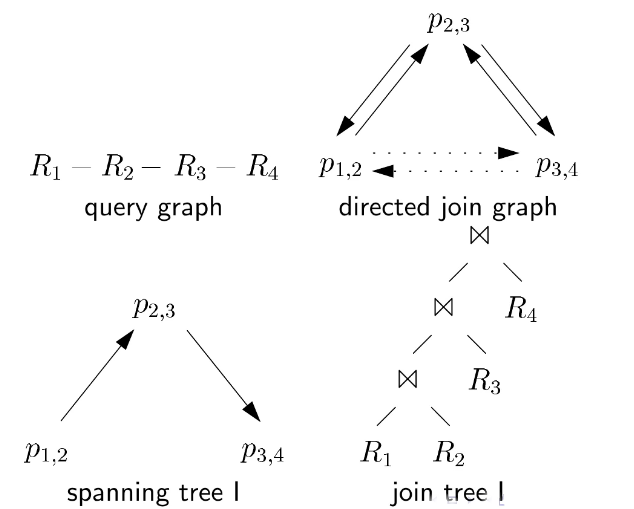
\includegraphics[width=0.48\textwidth]{MVP.png}
	\vspace{-50pt}
\end{wrapfigure}

For instance, every spanning tree in the directed join graph leads to a join tree: first of all edges are added in both direction, and then one of them gets removed, giving a directed acyclic graph which can easily give a join order (without distinguishing left and right).

MVP has the advantage of also producing bushy trees, however it does not guarantee optimality of the spanning tree; furthermore, the output might not correspond to an effective join tree.

Despite the incorrect representation, it is simple to fix this kind of errors, but there is no specific way to produce the best join tree.

To remedy the uncertainty, some additional rules are introduced to identify an effective spanning tree. The following conditions must be satisfied:
\begin{enumerate}
	\item $T$ must be binary (no nodes can have more than two children);
	\item For all inner connected nodes $(u, v)$, $R(T(u)) \cap R(v) \neq \emptyset$ (they must have predicates in common);
	\item For all $(u_1, v)$, $(u_2, v)$ one of the following holds:
	\begin{enumerate}
		\item $((R(T(u_1)) \cap R(v))) \cap ((R(T(u_2)) \cap R(v))) = \emptyset$ (they have a different relation in common);
		\item $(R(T(u_1)) = R(v)) \land (R(T(u_2)) = R(v))$ (the relations in common are the same between pairs).
	\end{enumerate}
\end{enumerate}
An effective spanning tree corresponds to a valid join tree, despite the definition not being intuitive. Given this, the rest of the assumptions is simple: if every predicate involves two relations and an equi-join condition, then $R(u) \cap R(v)$ contains only a single relation.

Let $v$ be that relation, then $R_i \bowtie_v R_j$ is abbreviated by $\bowtie_v$.

The next step is adding weight to the edges, obtaining a weighted directed join graph. Each weight is calculated with the formula:
$$w_{u, v} = \frac{\abs{\bowtie_u}}{R(u) \cap R(v)}$$
This means that each edge has a weight depending on the relation they have in common and the join cardinality. The intuition implies that a join is executes before another, the given relation becomes available and the edge weight can explain how the cardinality changes, i. e. how many tuples are generated.

This value can be bigger or smaller than 1, and can make the total cost bigger or smaller (the input size changes by a factor of $w_{u, v}$). For virtual edges, the weight is 1 by default. 

It is relevant to notice that the weight function used by MVP is the same one as $s_i$ in IKKBZ. However, it can also be chosen arbitrarily.

Of course, a weight smaller than 1 reduces the cost of following join operations. Furthermore, weights change over time depending on a partial spanning tree: 
$$w(p_{i, j}, S) = \frac{|\bowtie_{p_{i, j}}^S|}{\abs{R_i \bowtie_{p_{i, j}} R_j}}$$
$\bowtie_{p_{i, j}}^S$ is the result of the join after all joins preceding $p_{i, j}$ in $S$ have been executed. If the spanning tree is empty, the cost is merely equal to the cost of a simple join. 

\subsubsection{The algorithm}
The algorithm works in two phases:
\begin{enumerate}
	\item Taking the edges with weight smaller than 1, trying to reduce the work for latter operators as soon as possible;
	\item Adding the remaining edges, potentially causing an increase of the load, yet as late as possible.
\end{enumerate}
MVP takes as input a weighted directed join graph and builds two priority queues, one with largest weights (phase 1) and one with smallest (phase 2). 

The working graph is initially just a set of predicates with no edges, and then the two phases are ran.

The first phase modifies the state of a working tree, taking the head of the priority queue (the most expensive) and finding the joins which could make it cheaper, adding nodes with smaller weight while still keeping the graph acyclic.

If there is no such edge, the element is swapped from the first queue to the second; else, the edge to be added to the working tree will be the one which maximizes the difference within costs (minimizes the new cost). Weights are then recomputed. 

Phase 2 is called when the second queue is non-empty, again considering edges which respect the acyclic property. The procedure tries to minimize the additional cost caused by adding joins. 

To effectively modify the working tree, an update function changes the state by performing unions of sets with edges and removal from the graph yet to consider. If there are two incoming physical edges, they are replaced with virtual ones. 

This also ensures the binary property, removing all cases in which a node could have two parents and handling eventual duplicates. However, there is still no guarantee of optimality. 

\subsection{Dynamic Programming}
Dynamic programming approaches can be useful to obtain more insights on possible orders with cost function. Since this kind of algorithm is a macro class, they can be defined on any input and give any output (bushy, left-deep).

These work thanks to an optimality principle: if an option is cheaper than another, the latter can be discarded and the best solution is found only considering the set of further possibilities generated by the first.

Formally, let $T$ be an optimal join tree for relations $R_1, \dots, R_n$. Then, every subtree $S$ of $T$ is an optimal join tree for the relations contained in it.

Despite some hypothetical concerns of sub-optimality and the presence of physical properties which may alter the result, in practice this property holds.

\begin{wrapfigure}{L}{0.49\textwidth}
	\vspace{-10pt}
	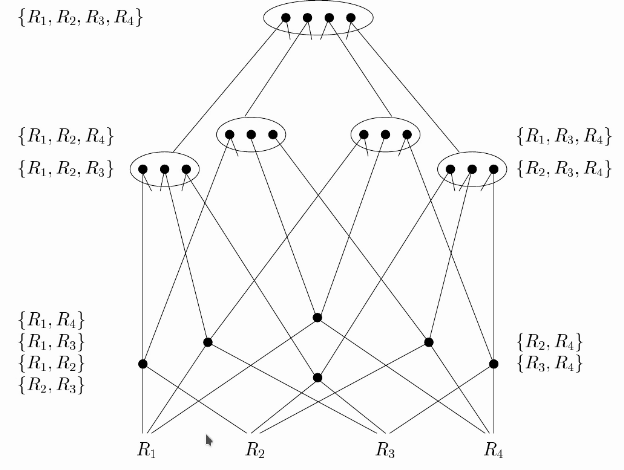
\includegraphics[width=0.5\textwidth]{search_space.png}
	\vspace{-40pt}
\end{wrapfigure}

The strategy works starting with a single relation and generating larger trees with a bottom-up strategy, reusing previous intermediate results.

A possible dynamic programming algorithm calculates the cost functions when joining either on the left or right side (bushy usually works better) for each applicable join implementation. 

The outcome will be a list of pairs with their cost, of which the minimum is chosen and propagated through following iterations.

The search space gets therefore reduced whenever an option is discarded, hence the number of combinations is never exponential.

In the case of linear trees, there is a basic strategy finding the optimal $T$ by joining all optimal $T'$ with $T \setminus T'$, with $|T| = |T'| + 1$.

The most common algorithm constructs the optimal left-deep tree from an empty table mapping the set of relations ($2^R$) to the join tree. 

For each relation, the optimal tree is built, starting from size 1 and increasing the subsets by adding those of smaller size having the optimal solution of the subproblem.

If $S$ is a subset of $\{R_1, \dots, R_n\}$, before a join tree for it can be generated, the join trees for all relevant (valid) subsets of $S$ must already be available.

For instance, if the query graph is a chain, before computing the optimal order there must be calculations for each connected pair, and of course for single relations.

Running time depends on the number of combinations: DP-sub is slower in the polynomial case.

\subsubsection{Integer order}
Integer order is a numeration used to order relations instead of the size.

This representation can be seen as a binary number in which a digit is 1 if the set contains the relation corresponding to its position, and 0 otherwise. For instance, having three relations, $011$ is $\{R_1, R_2\}$.

An alternative algorithm to generate linear trees uses integer order to fill the dynamic programming table, calculating all combinations for each $2 \leq i \leq 2^n-1$ and finding all subsets such that their binary representation is 1.

The real implementation does not perform any mathematical operation, since each $i$ already represents a set. 

Then, for each relation in the subset, the cost is added to smaller sub-problems, similarly to the previous approach. The last bit of the set gets removed after every iteration.

This algorithm has even better performance when creating bushy trees, and its advantage is the speed of binary calculations (bitwise and). 

\subsubsection{Bushy trees}
Bushy trees can be generated by combining two optimal trees (children of newly-found node). The dynamic programming principle holds.

A basic strategy is in fact just optimizing over sub-problems and aggregating them: the approach is similar to linear trees, with the variant that the combined size of each pair of intermediate result must be equal to $\abs{S}$. Every relation must also appear once, hence $S_1 \cap S_2 = \emptyset$.

In practice, the number of subsets is exponential, and most of the time sizes are not compatible: a possible implementation uses a linked list of all combinations, and edits it according to the next operation.

Integer order is particularly efficient since the complement of a set ($S_2 = S \setminus S_1$) is found in constant time when the representation is binary.

All subsets can be enumerated as follows:
\begin{lstlisting}[language=C++]
S_1 = S & (-S)  // gives a number having only 1 as last bit
do {
	S_2 = S - S_1
	S_1 = S & (S_1 - S)  // same meaning as plus
} while (S_1 != S)
\end{lstlisting}
Computational time is quite low, which is useful for a large amount of relations.

\subsection{Memoization}
Memoization is a top-down formulation of dynamic programming, recursively generating join tree in a way which allows to avoid duplicate works and to prune useless solutions.

Code is easier to understand and sometimes more efficient, but usually slower due to recursiveness.

The memoization algorithm fills the table and then performs an auxiliary procedure for each subset: it checks whether the problem has already been computed, otherwise it splits the subset in two and recursively calculates the two values.

At the end of all function calls, the best value is picked between the two and the cost is returned. 

The most performance-critical operation is the lookup in the hash table of known combinations, which can be expensive making the whole procedure slow.

The advantage is the knowledge of a cost boundary immediately after the first loop, meaning that in further iterations it is possible to propagate values so that more expensive plans can be discarded.

However, eliminating solutions might prune other optimal combinations or force sub-optimal sets: the table must be extended, also remembering failures, so that it is not necessary to run the procedure another time.

The cost boundary can grow exponentially: a rule of thumb would be doubling it when searching for solutions and so on, ensuring a limited number of tries. 

\subsection{Connected subgraphs}
Connected subgraphs are another alternative to dynamic programming taking into account the structure of the query graph and the connectivity of nodes.

For large queries, it is not quite efficient to construct sub-problems which will be discarded later since they do not correspond to a valid tree. On the other side, it is possible to argue that pruning typically removes invalid subsets.

Having the query graph also helps to reduce asymptotic search space (polynomial) for chains, while it does not work well for cliques (exponential). Dynamic programming is instead better for cliques, but scales badly.

However, chains or quasi-chains are the most common kind of graph in real-world applications of joins, so the first approach is more useful in practice.

Join ordering formulated as a graph theoretical problem works with the following steps:

\begin{enumerate}
	\item Enumerating all connected subgraphs among the query graph;
	\item Enumerating all subsets which are disjoint but connected to the subgraph which is being considered;
	\item Trying to join each connected subgraph with its complement pair;
	\item Finding suitable combinations (DP algorithm).
\end{enumerate}

This approach can be merged with DP so that the latter works with already enumerated subgraphs, making it easier to get rid of invalid solutions.

This allows tight polynomial lower bounds which are currently optimal. 

However, pairs have to be enumerated correctly and efficiently: this is a two-step procedure starting from the subsets and reaching supersets, avoiding commutative pairs and assuming a total order of connected subgraphs (to guarantee avoidance of duplicates).

A total order is achieved by labeling nodes through a breadth-first search. After this preparatory step, the actual algorithm can start having available all nodes along with their neighborhood (nodes reached with an edge). Furthermore, each set has a block composed by nodes coming before, to avoid enumerating twice.

All nodes are considered in descending order and emitted (since each is a connected subgraph), then the graphs are recursively expanded prohibiting nodes with smaller labels. 

Expansion is performed similarly to DP-sub, looking in the neighborhood among possible combinations. The set of valid nodes increases over time, allowing more degrees of freedom.

To achieve idealistic runtime, set operations should be performed in constant time, but in the general case this is not expected and a linear delay might happen; in practice, values are encoded as integers to gain speed, yet this only works in the order of 64 relations.

Another solution is using bitsets, implementations with dynamic memory and variable size. This does not guarantee constant time either, even if allocating enough bits should never cause a resize.

\subsection{Complex queries}
There are cases in which the query graph is particularly complicated, such as $abs(r_1.f + r_3.f) = abs(r_4.g + r_6.g)$. This kind of operation generates a hyper-graph, connecting more than two relations at once: common algorithms cannot be applied. DPSize does not consider the query graph, so it could be used, but it does not have optimal runtime.

A hypergraph is a non-empty set of nodes and edges where a hyperedge is an unordered pair of non-empty proper subsets with empty intersection. They have a total order via an arbitrary relation, to avoid enumerating multiple times, or breadth-first search.

The approach is similar as for regular graphs, starting with one node and recursively expanding. However, hyperedges have a many-to-many relationship, and an additional choice of where to expand must be taken, while still guaranteeing DP order. The DP table can be tested to check if nodes into subsets are connected, implying an entry already exists. 

For instance, it is impossible to join a set of relations with only one relation which is connected by a hyperedge, since it means some information is lacking and a cross product would be necessary. Therefore, the single relation is recursively expanded checking for connections.

A minor change to solve this issue is choosing a representative for each hyperedge, leading to the last node in total order, so that duplicates are prevented. Checks for connectedness are still required, because this method leads to temporarily disconnected graphs which must be further expanded.

Another interesting case involves non-inner joins (either outer or unnesting), not freely reorderable (performing an inner join before an outer will reduce the number of output tuples, and vice versa). 

There are compatibility matrices stating whether two join operations are commutative assuming syntax constraints, i. e. $(R \circ_1 S) \circ_2 T \equiv R \circ_1 (S \circ_2 T)$. For instance, full outer joins can be swapped with themselves. 

Using this information, it is easy to figure out which operations are permitted. For each operator, the syntactic eligibility set (SES) is built, a set of relations which must be in the input; then, the total eligibility set (TES) is constructed in a bottom-up way, starting with SES and checking for conflicts in selectivity. If this is the case, another TES is added, capturing reordering restrictions. 

The output obtained adding TES encodes the necessity of certain relations while constructing hyperedges, eliminating invalid reorderings.

\subsubsection{Simplifying the query graph}
The dynamic programming approach always considers minimal number of join-pairs, so it is not expected to get a better runtime for exact solutions. The set of possibilities is limited, and algorithms perform slowly for certain query graphs (stars), but the complexity is most likely the best to be achieved.

There are ways to recognize whether the problem is too complicated to be solved with DP, and simplify (from an optimizer point of view) the query graph until it gets tractable. 

Some possibilities of course are going to be ruled out if edges are removed, hence safe modifications are preferred, using a greedy method for simpler problems and then performing DP on intermediate results. 

To effectively decrease the search space size, some joins (shrinking) can be forced to be performed first, halving the number of potential plans with each restriction. 

The steps to be performed are:
\begin{enumerate}
	\item Examine all joins that have a relation in common (neighboring);
	\item Check that a pair can be swapped of order (needs a fast cycle checker, trying to construct a topological ordering);
	\item Compute the ordering benefit with different heuristics;
	\item Retain the pair with maximal ordering benefit, maintaining priority queues to speed up repeated simplification;
	\item Return the query graph in which the edge corresponding to the join is changed.
\end{enumerate}
This method is more restrictive, hence simpler. 

The ordering benefit can be estimated in several ways. One approach is to maximize the following:
$$\text{orderingBenefit}(X \bowtie_1 R_1, X \bowtie_2 R_2) = \frac{C((X \bowtie_1 R_1) \bowtie_2 R_2)}{C((X \bowtie_2 R_2) \bowtie_1 R_1)}$$
$C$ is an arbitrary cost function, for instance $C_{out}$ when no other information is available.

The program should also know when to stop simplifying: this is achieved when memory or time constraints are satisfied, along with counting the number of connected subgraphs or bounding through memory consumption.

Counting is fast, but not immediate, and cannot be performed after every simplification: a reasonable choide is 10 000 connected subgraphs.

The full optimization algorithm runs first of all computing a list of query graphs, in which the elements are the same graph after each step, performing simplifications until a total order is reached; to find a specific plan, binary search is employed and then DPhyp is ran on each of them.

After the optimal simplification is obtained, dynamic programming is used to get the ultimate result.

Simplification heuristics are subject to mistakes, hence performing too many probably means at some point the cost will increase, and it would be best to stop earlier. This problem is NP-hard.
